\subsection{\ystar\ cut Optimization}
\label{section:ystarCutOptimization}

\todo[inline]{ Clean up formulae. }

In QCD two-to-two scattering, $t$-channel is dominant. The QCD dijet production is proportional to 
$\displaystyle{(1-\cos\theta^{*})^{-2}}$, while $H^\prime$ and String production is expected to be flat in 
$\cos\theta^{*}$. This means that \ystar\  of QCD background will minimize at 0 and that of $H^\prime$  
and String will peak at 0.


The significance is given by 
\begin{equation}
\label{eq:signifcanceYstar}
S  = \sqrt{\sum_{i}{2\left[ \left(S_{i}+B_{i} \right)\cdot \ln \left(1+\frac{S_{i}}{B_{i}}\right)-S_{i}\right]}}
\end{equation}
where $S_i$ ($B_i$) is the number of signal (background) events in bin $i$. 
Figure \ref{fig: hprime significance as a function of y* cut} shows $H^\prime$ signal significance as a function 
of the value of the \ystar\  cut. The significance peaks  around 0.6, so the optimal $y^{*}$ cut for the $H'$ search is 
$|\ystar| < 0.6$. Figure \ref{fig: string significance as a function of y* cut} shows the String signal significance as a function of \ystar\ cut. The significance peaks at  0.8, so the optimal  cut for the String search is $|\ystar| < 0.8$.

\begin{figure}[htbp]
        \centering
        \subfigure[$\geq$1 g-tag]{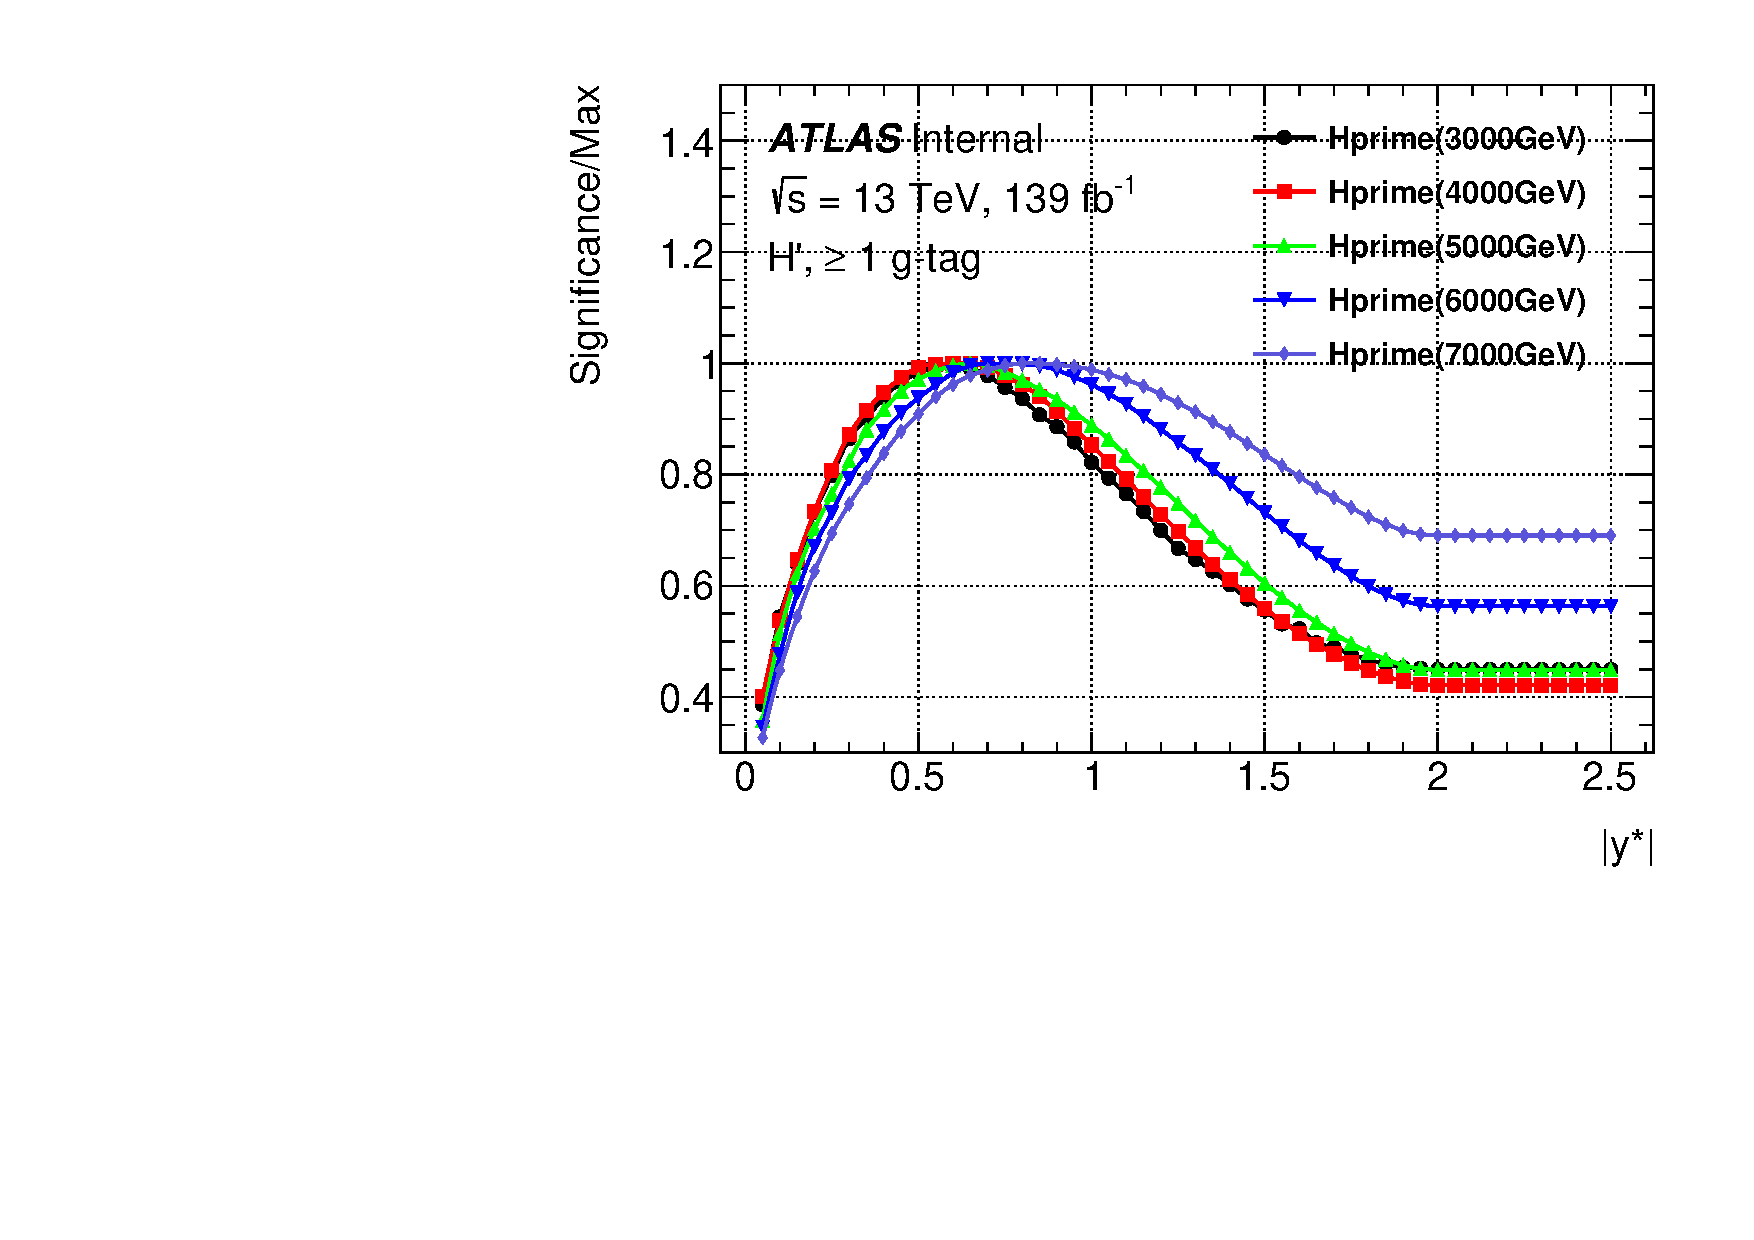
\includegraphics[width=0.48\columnwidth]{figures/yStarOptimization/Significance_Hprime_gj.pdf}}
        \subfigure[2 g-tag]{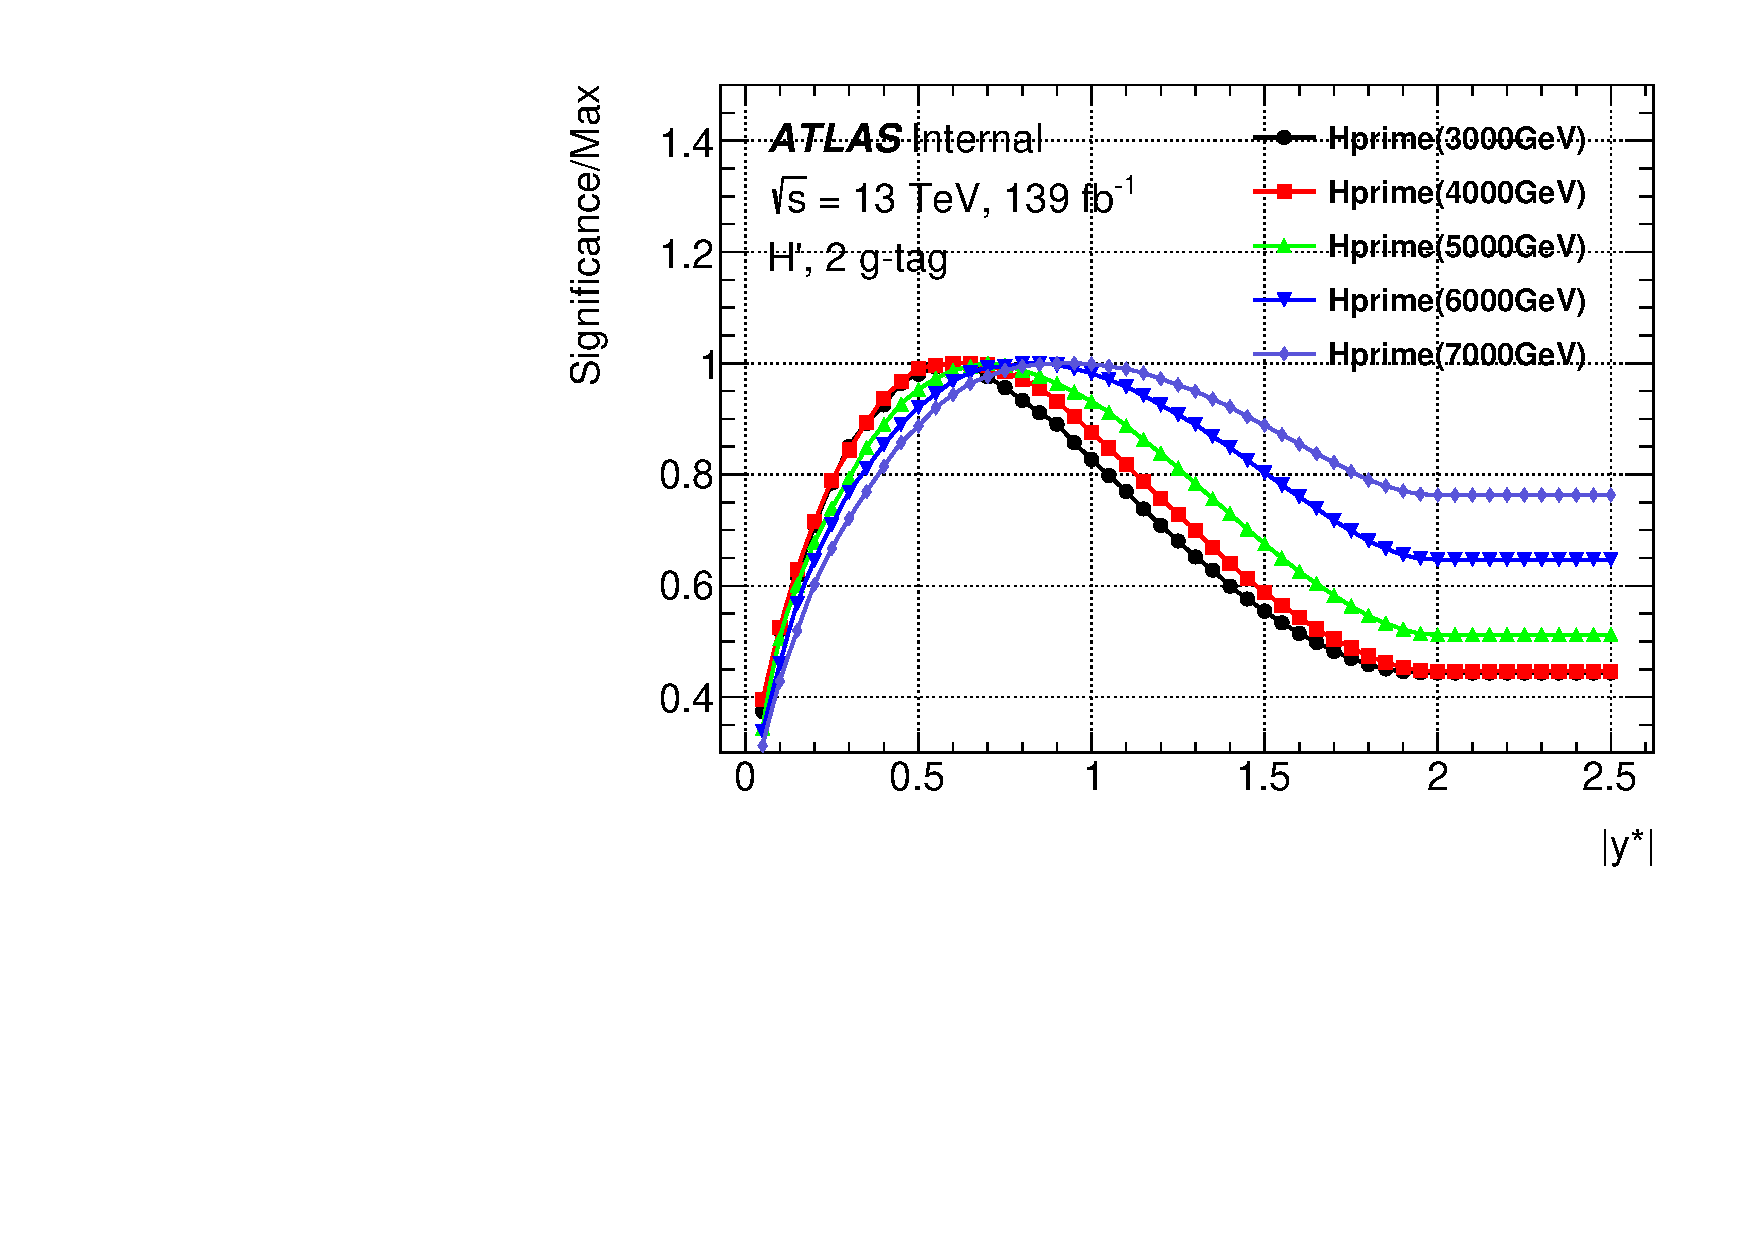
\includegraphics[width=0.48\columnwidth]{figures/yStarOptimization/Significance_Hprime_gg.pdf}}
        \caption{$H^\prime$ significance as a function \ystar\ cut in the case of (a) $\geq$1 g-tag, (b) 2 g-tag.}
        \label{fig: hprime significance as a function of y* cut}
\end{figure}


\begin{figure}[htbp]
        \centering
        \subfigure[$\geq$1 g-tag]{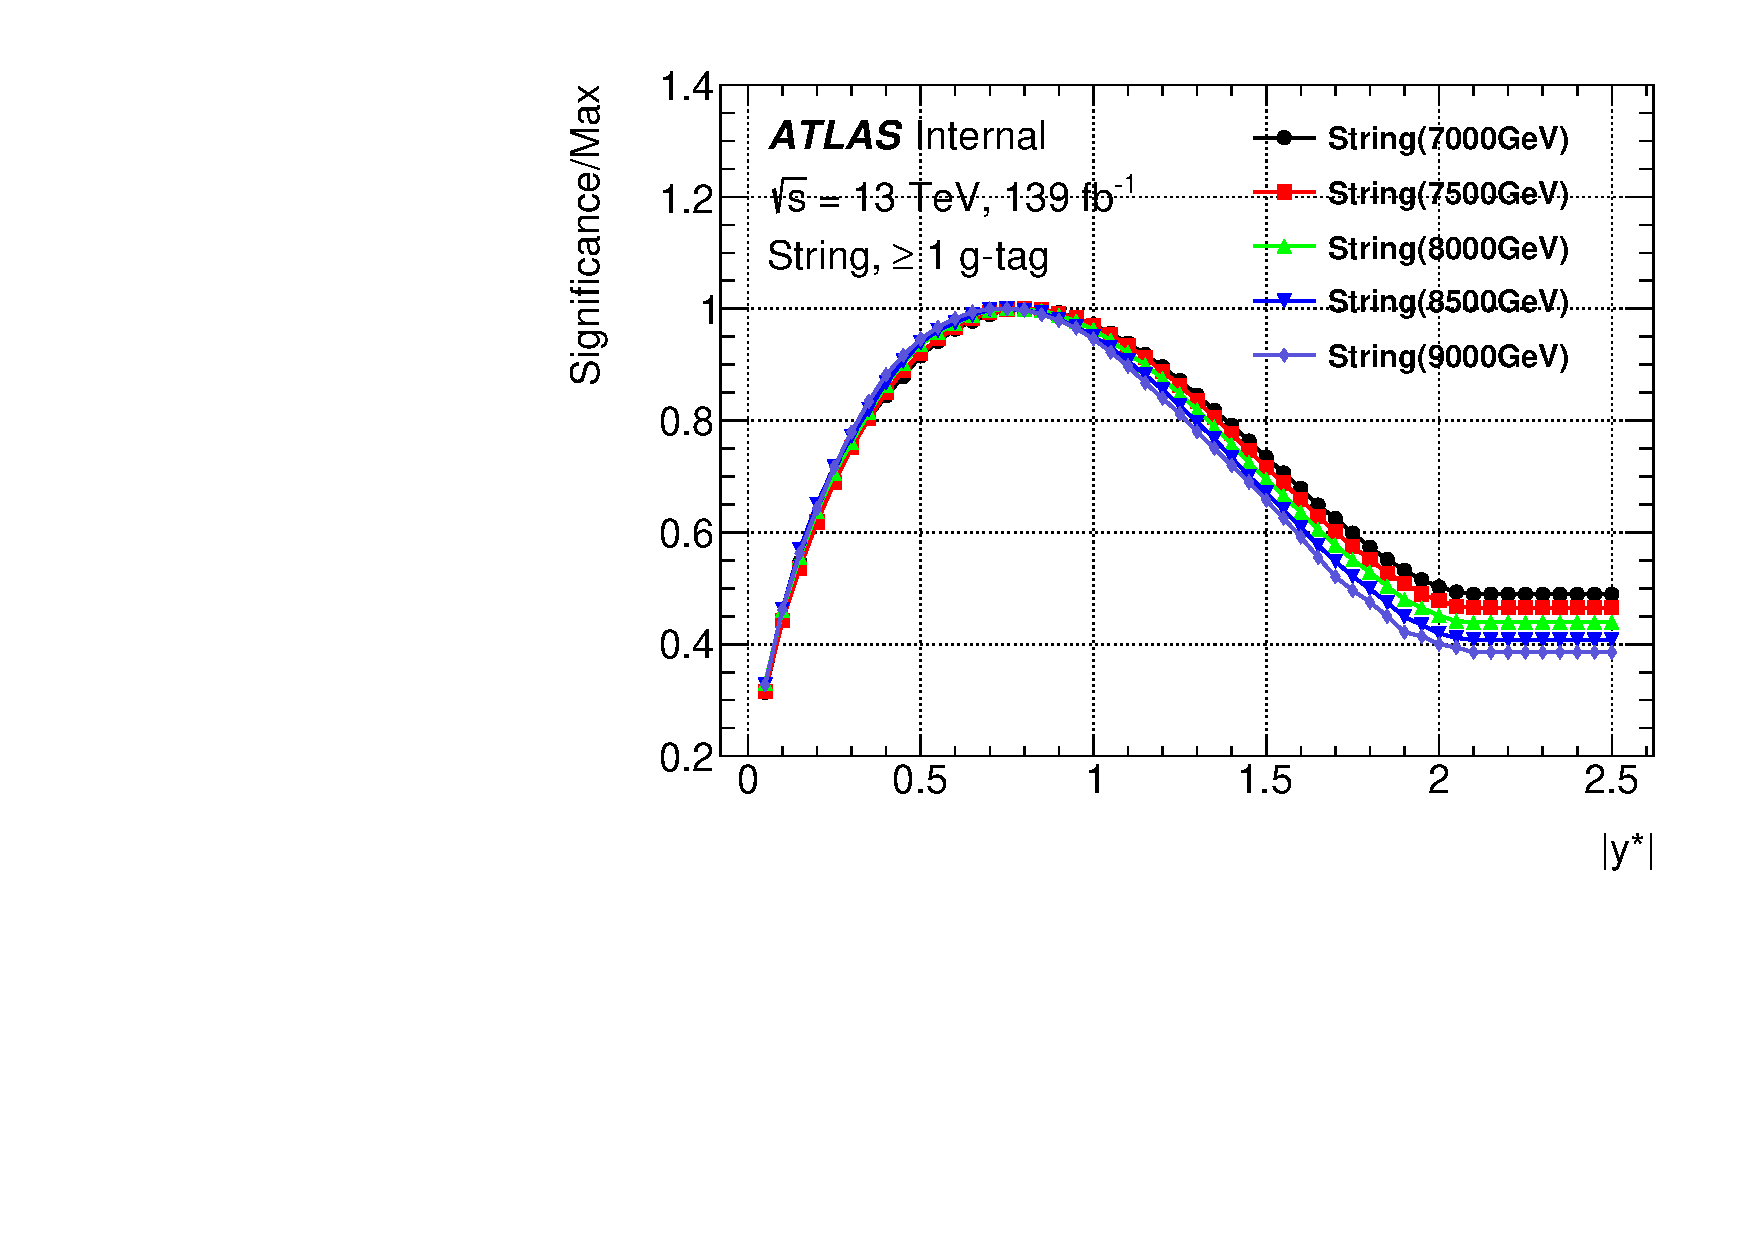
\includegraphics[width=0.48\columnwidth]{figures/yStarOptimization/Significance_String_gj.pdf}}
        \subfigure[2 g-tag]{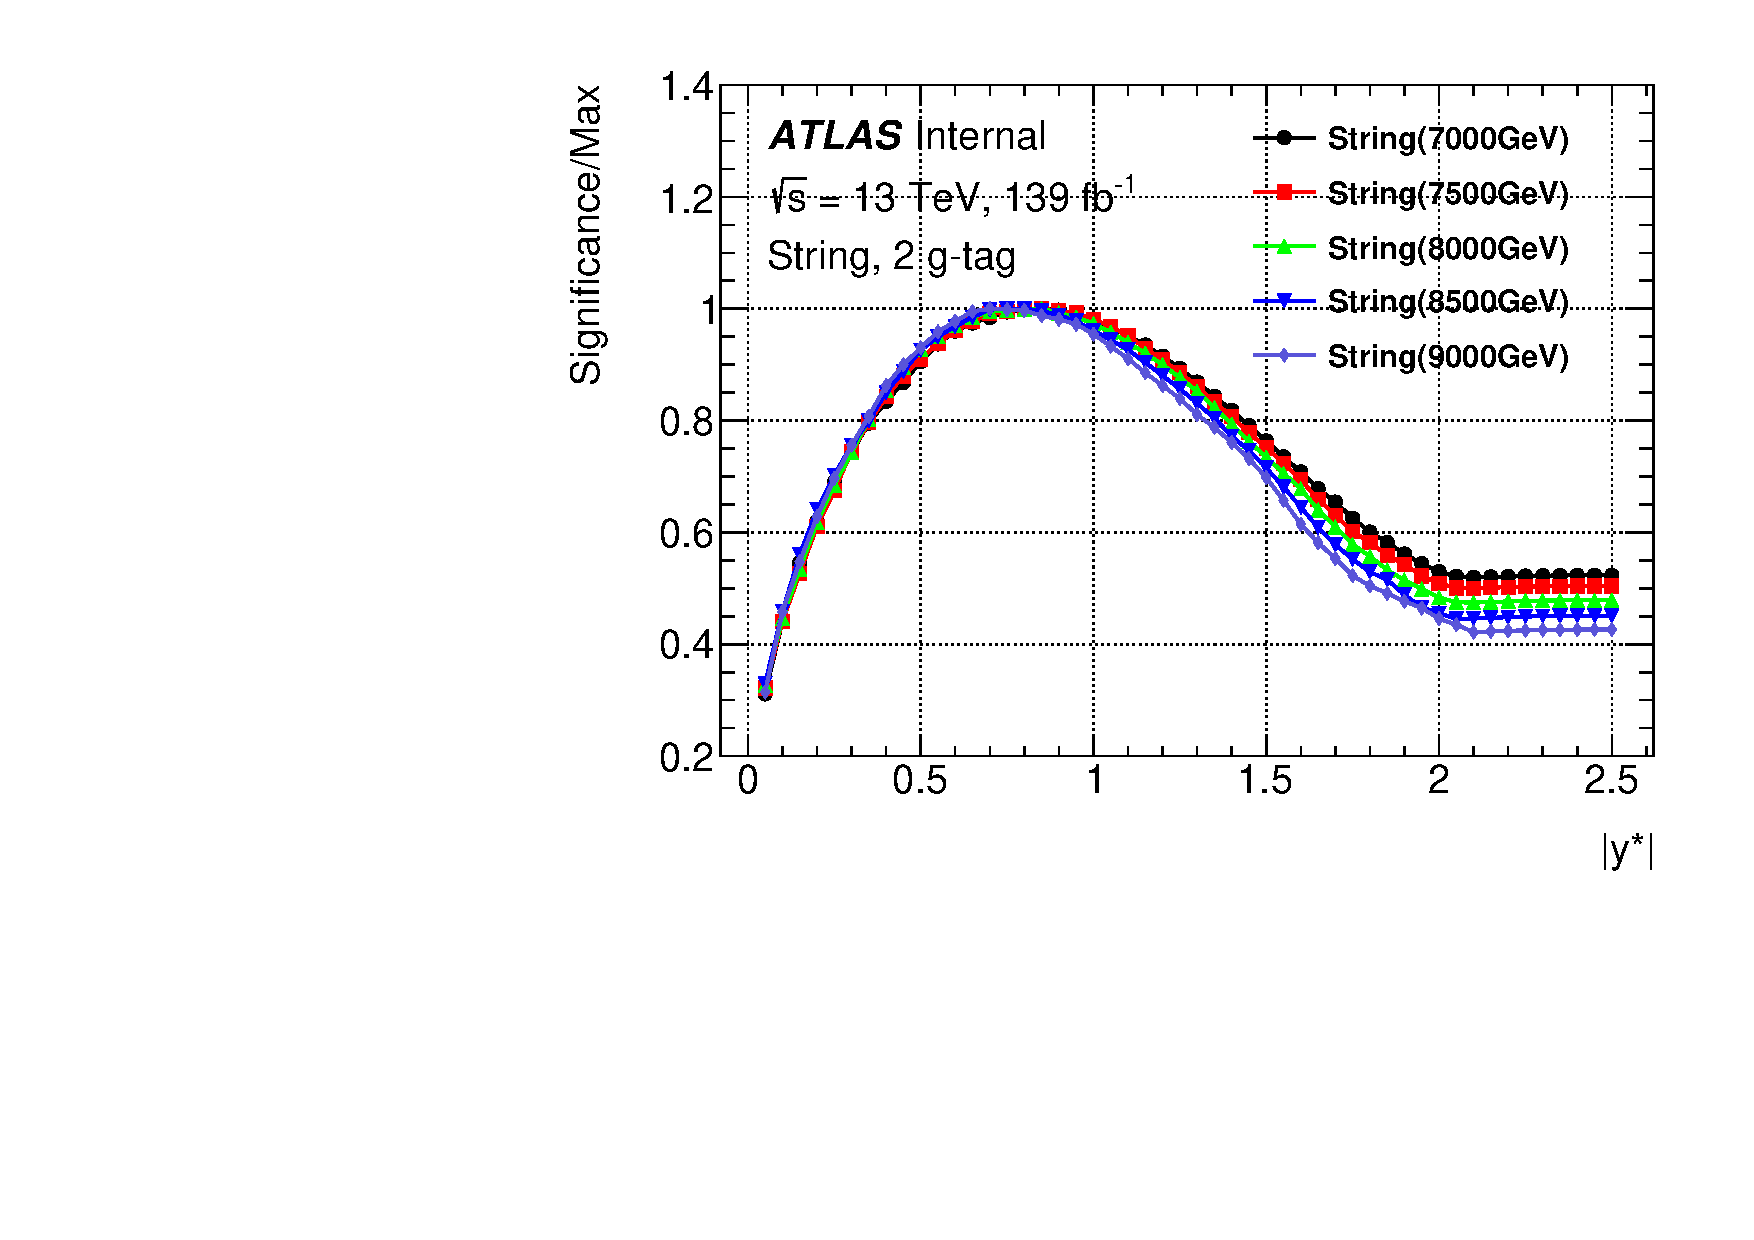
\includegraphics[width=0.48\columnwidth]{figures/yStarOptimization/Significance_String_gg.pdf}}
        \caption{String significance as a function \ystar\ cut in the case of (a) $\geq$1 g-tag, (b) 2 g-tag.}
        \label{fig: string significance as a function of y* cut}
\end{figure}




\subsection{dijet mass turn-on}
\label{section: dijet mass turn-on}

The lowest single jet un-prescaled trigger in 2015 was HLT\_j360, in 2016 was HLT\_j380,
in 2017 and 2018 is HLT\_j420 which is available in full Run 2 data.
A mass cut will be applied to remove events where the trigger efficiency is less than 99.5\%.

To measure the \mjj\ turn-on in data, an unbiased sample was obtained using the HLT\_j360 trigger, 
only data collected in 2015 corresponding to 3.2\,\ifb\ is used in this measurement.

Figure \ref{fig: mass turn-on yStar 0.6} shows the efficiencies as a function of \mjj\ for $|\ystar|<0.6$ in two g-tag regions for both triggers. The \mjj\ value of the plateau ($\geq$99.5\%) is 1100\,\GeV. Figure \ref{fig: mass turn-on yStar 0.8} shows the efficiencies as a function of \mjj\ for $|\ystar|<0.8$ in two g-tag regions, the plateau value is 1200\,\GeV.

\begin{figure}[htbp]
        \centering
        \subfigure[$\geq$1 g-tag]{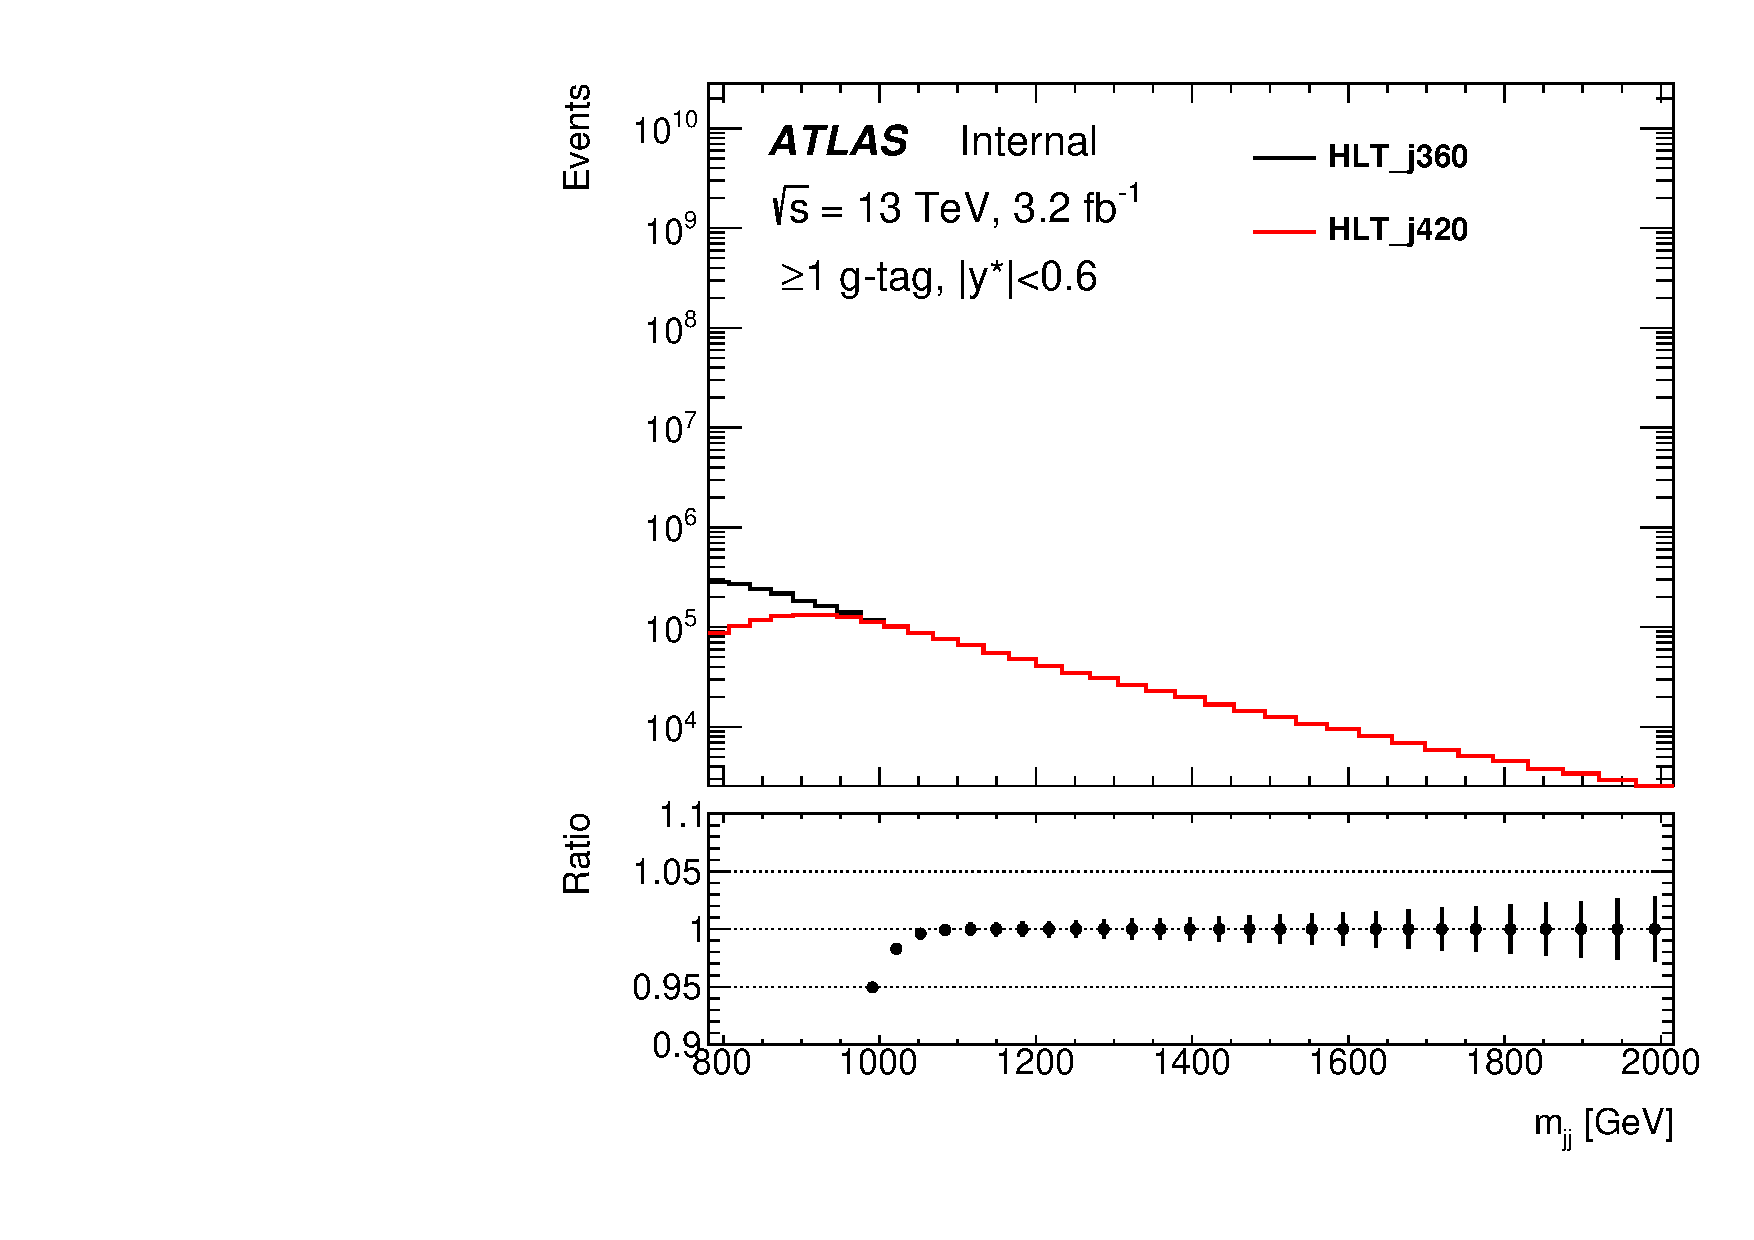
\includegraphics[width=0.48\columnwidth]{figures/massturnon/h_mass_gj_yStar0p6_ratio.pdf}}
        \subfigure[2 g-tag]{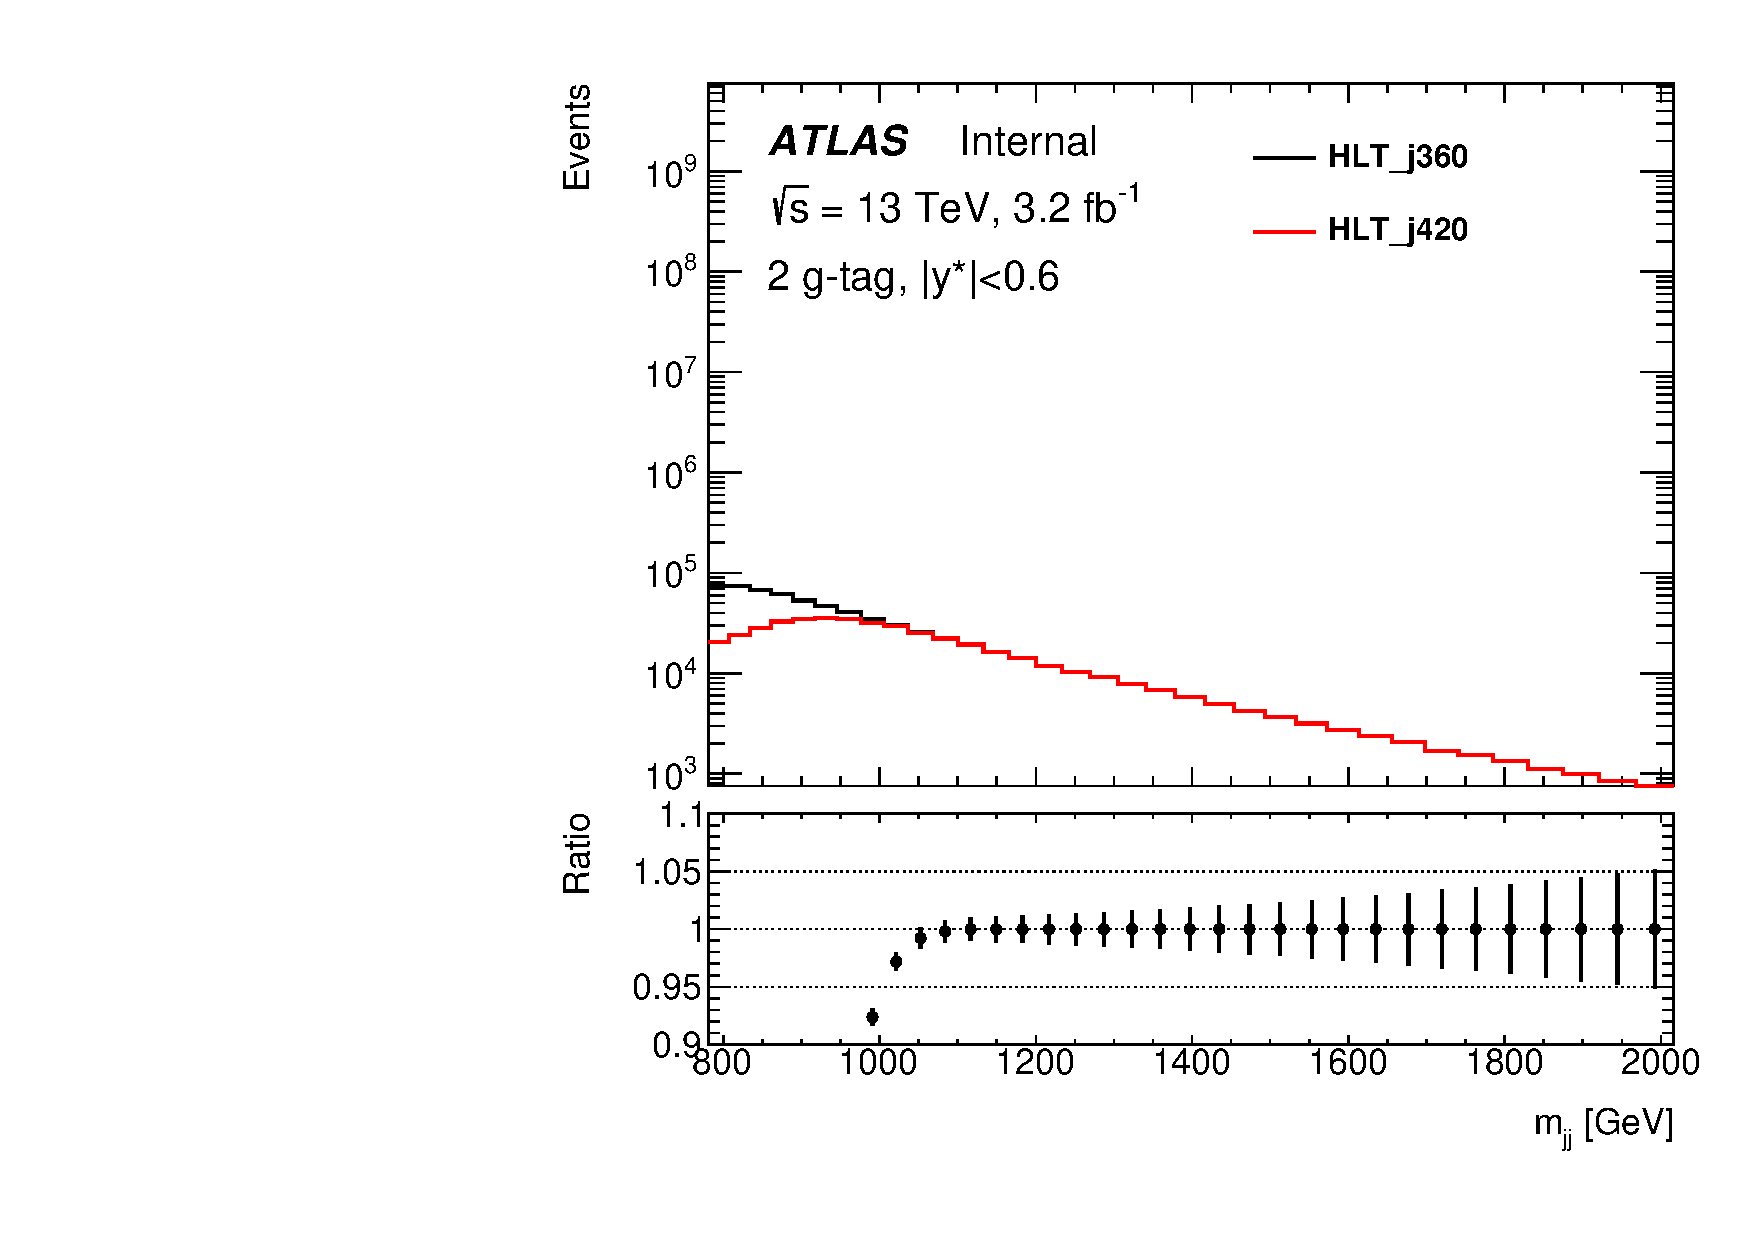
\includegraphics[width=0.48\columnwidth]{figures/massturnon/h_mass_gg_yStar0p6_ratio.pdf}}
        \caption{Efficiencies as a function of \mjj\ for $|\ystar|<0.6$ using HLT\_j420 in the case of (a) $\geq$1 g-tag, (b) 2 g-tag.}
        \label{fig: mass turn-on yStar 0.6}
\end{figure}

\begin{figure}[htbp]
        \centering
        \subfigure[$\geq$1 g-tag]{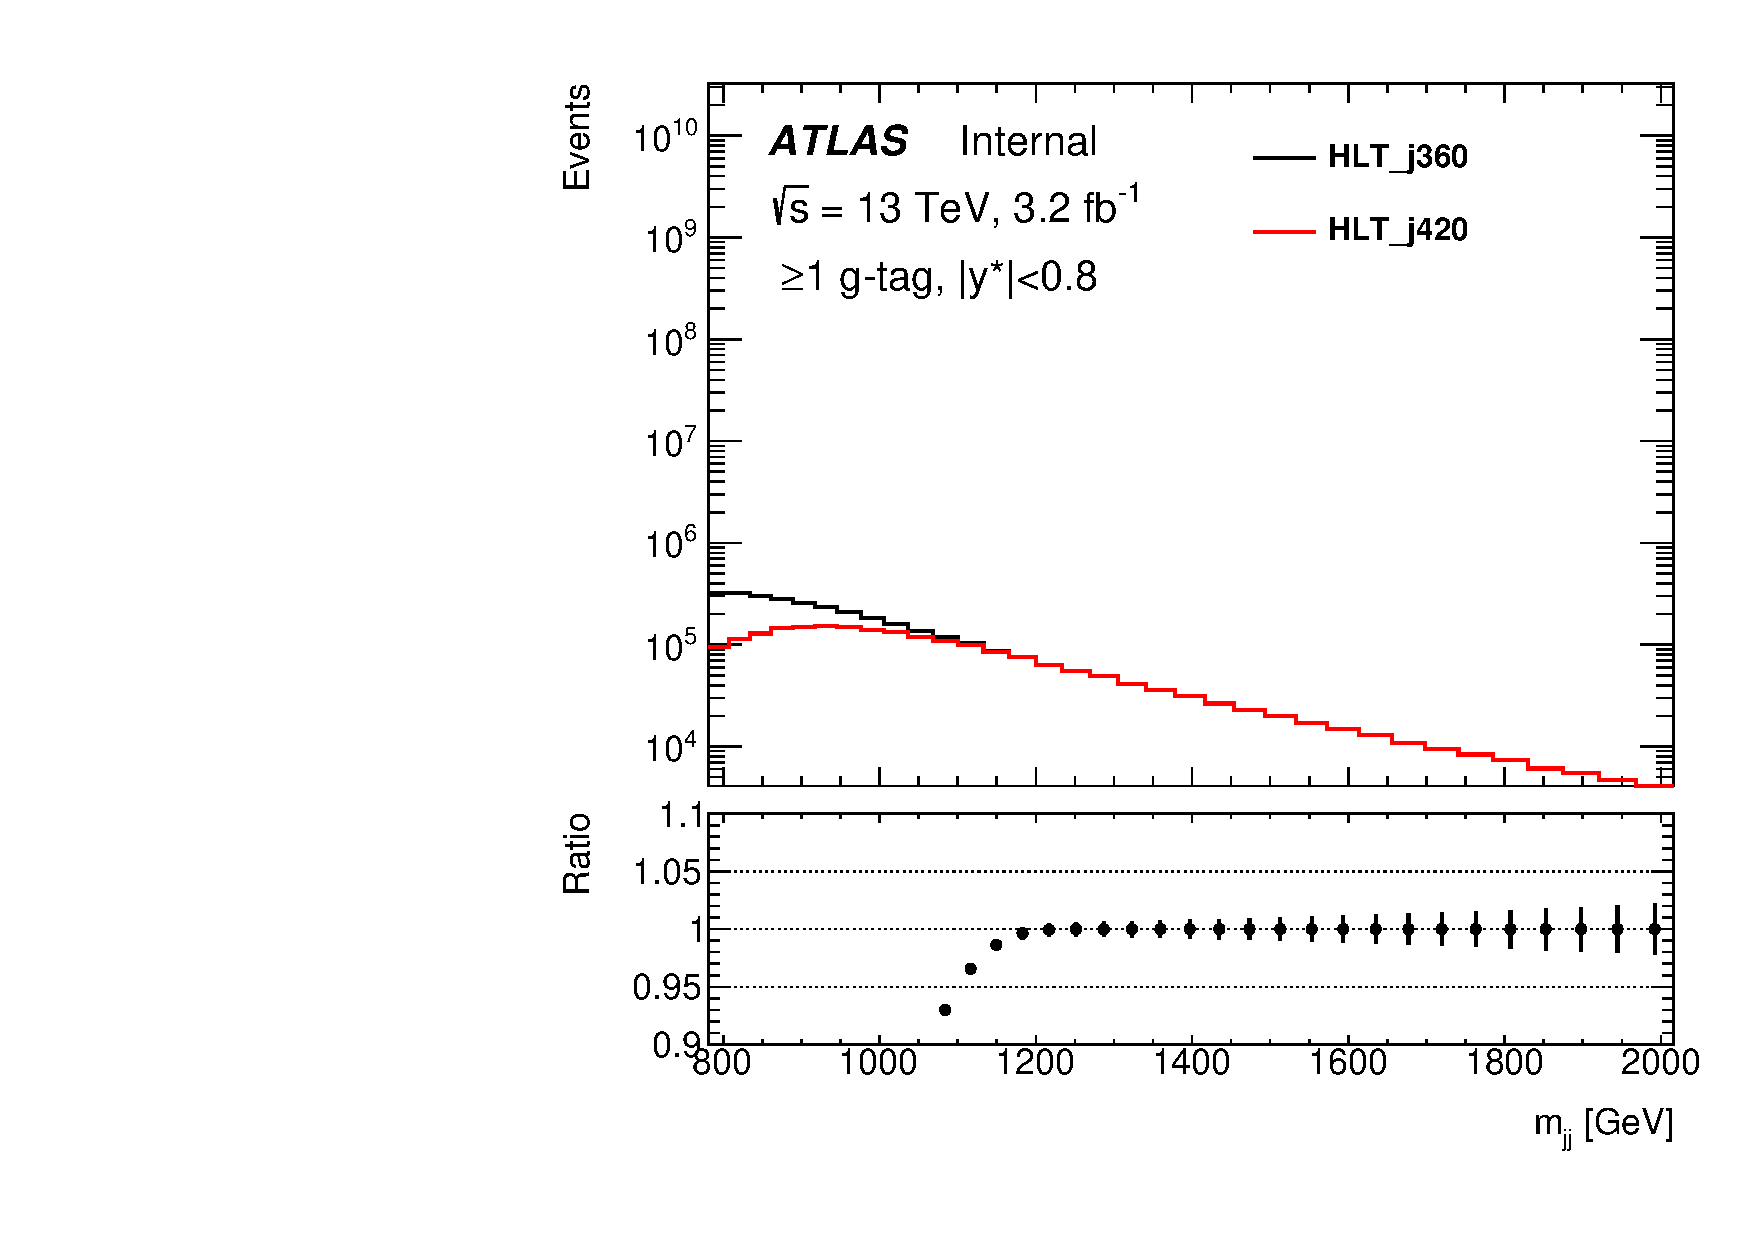
\includegraphics[width=0.48\columnwidth]{figures/massturnon/h_mass_gj_yStar0p8_ratio.pdf}}
        \subfigure[2 g-tag]{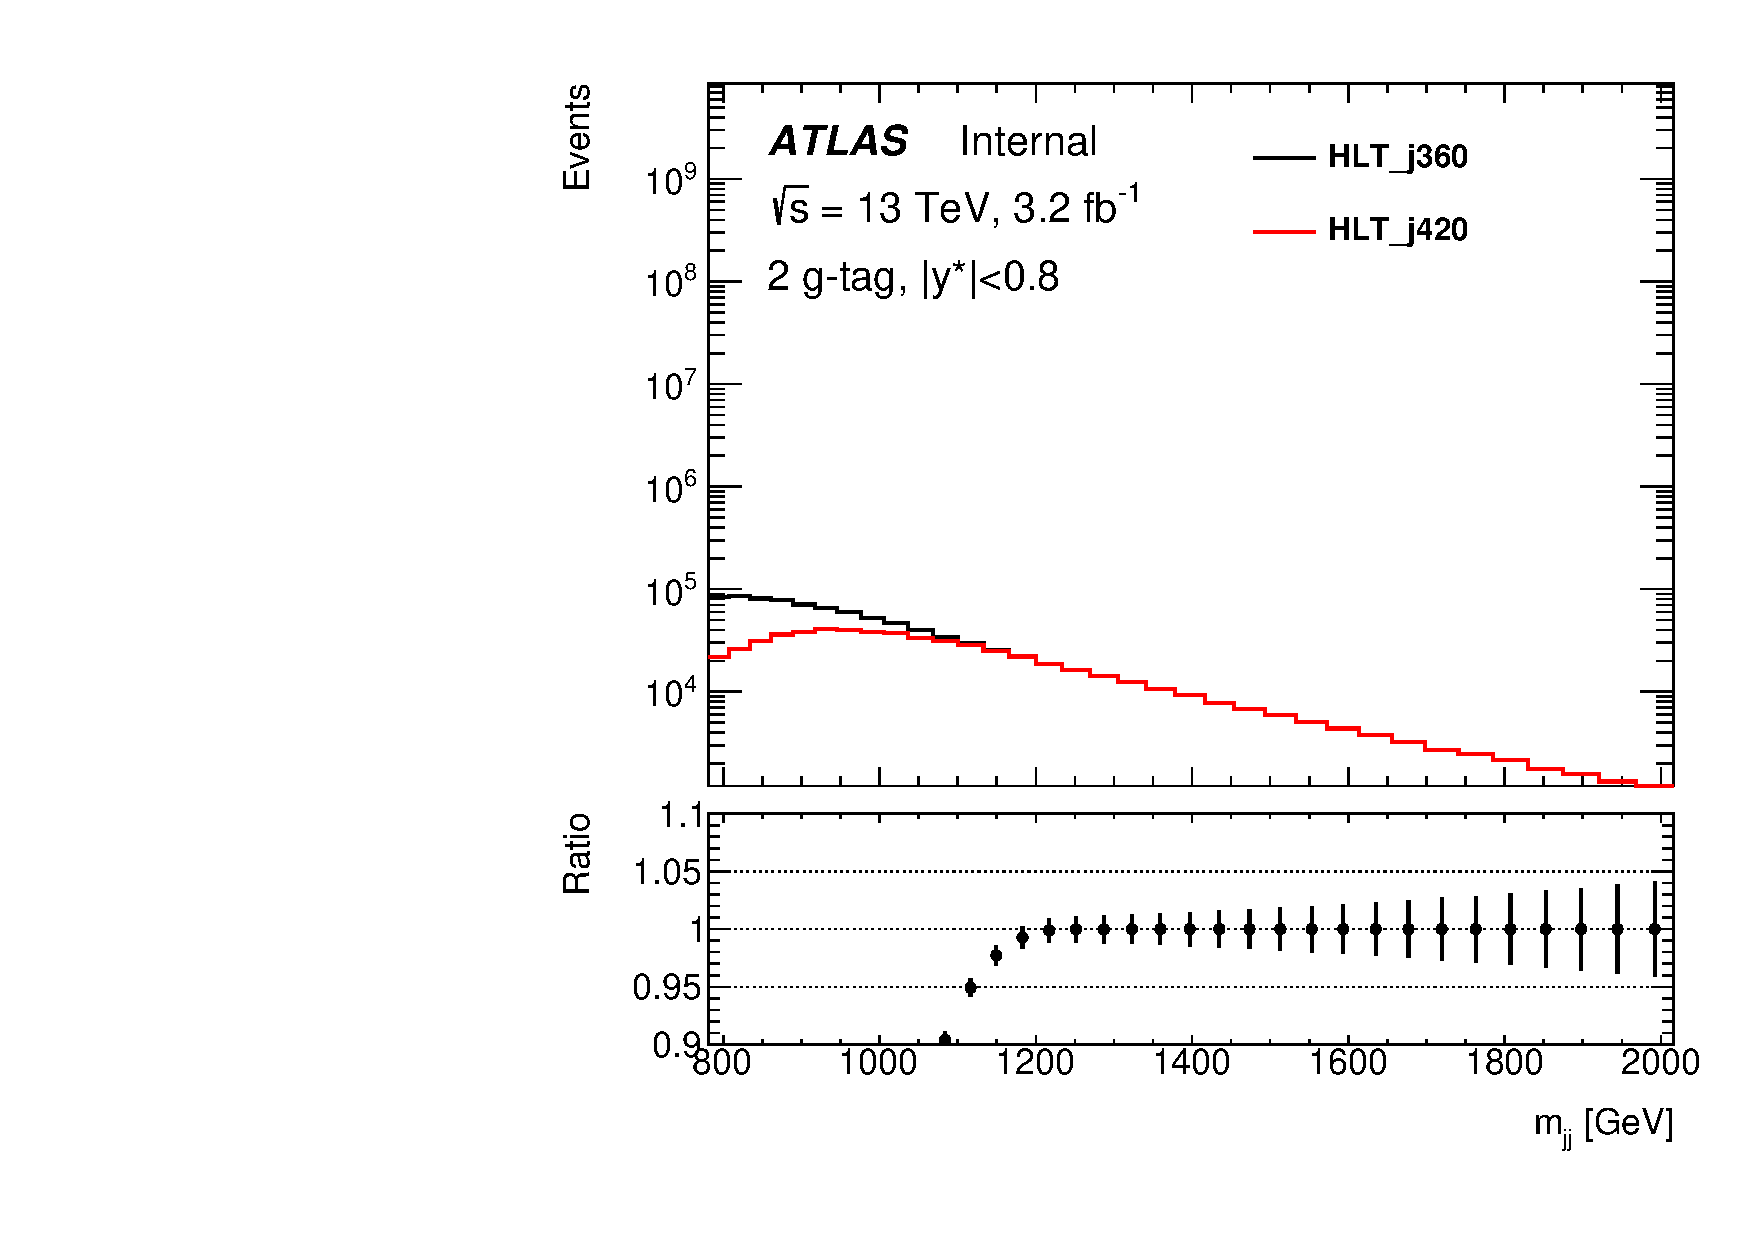
\includegraphics[width=0.48\columnwidth]{figures/massturnon/h_mass_gg_yStar0p8_ratio.pdf}}
        \caption{Efficiencies as a function of \mjj\ for $|\ystar|<0.8$ using HLT\_j420 in the case of (a) $\geq$1 g-tag, (b) 2 g-tag.}
        \label{fig: mass turn-on yStar 0.8}
\end{figure}

\subsection{Baseline selection}
\label{sec:base_selection}
The baseline event selection is applied for all signal regions and
the cuts applied are:
\begin{itemize}
\item Good Run List (GRL): Requirement that all relevant detectors were in a good state ready for physics. The GRLs used for this analysis are:
	\begin{itemize}
		%\item 2015(3.2\,\ifb): data15\_13TeV.periodAllYear\_DetStatus-v89-pro21-02\_Unknown\_PHYS\_ \newline StandardGRL\_All\_Good\,\_25ns.xml
		%\item 2016(32.97\,\ifb): data16\_13TeV.periodAllYear\_DetStatus-v89-pro21-01\_DQDefects-00-02-04\_ \newline PHYS\_StandardGRL\_All\_Good\_25ns.xml
		%\item 2017(44.31\,\ifb): data17\_13TeV.periodAllYear\_DetStatus-v99-pro22-01\_Unknown\_ \newline PHYS\_StandardGRL\_All\_Good\_25ns\_Triggerno17e33prim.xml
		%\item 2018(59.94\,\ifb): data18\_13TeV.periodAllYear\_DetStatus-v102-pro22-04\_Unknown\_PHYS\_ \newline StandardGRL\_All\_Good\_25ns\_Triggerno17e33prim.xml
                \item 2015(3.2\,\ifb): data15\_13TeV.periodAllYear\_DetStatus-v89-pro21-02\_Unknown\_PHYS\\\_StandardGRL\_All\_Good\_25ns.xml
        	\item 2016(33\,\ifb): data16\_13TeV.periodAllYear\_DetStatus-v89-pro21-01\_DQDefects-00-02-04\_PHYS\\\_StandardGRL\_All\_Good\_25ns.xml
        	\item 2017(44.2\,\ifb): data17\_13TeV.periodAllYear\_DetStatus-v99-pro22-01\_Unknown\_PHYS\\\_StandardGRL\_All\_Good\_25ns\_JetHLT\_Normal2017.xml
        	\item 2018(58.5\,\ifb): data18\_13TeV.periodAllYear\_DetStatus-v102-pro22-04\_Unknown\_PHYS\\\_StandardGRL\_All\_Good\_25ns\_Triggerno17e33prim.xml
	\end{itemize}
\item LAr: Liquid Argon Calorimeter error rejected ( errorState(xAOD::EventInfo::LAr) )
\item Tile: Tile Calorimeter error rejected ( errorState(xAOD::EventInfo::Tile) )
\item SCT: SCT single event upsets rejected ( errorState(xAOD::EventInfo::SCT) )
\item Core: Incomplete event build rejected ( isEventFlagBitSet(xAOD::EventInfo::Core, 18) )
\item All jets with $\pt\ge 150\,\GeV$ pass LooseBad cleaning cuts
\item Primary Vertex: the highest $\sum\pt^{2}(trk)$ (xAOD::VxType::VertexType::PriVtx) vertex has at least two tracks associated with it
\item Trigger: Passes the lowest unprescaled single-jet trigger, HLT\_j420
\item Jet preselecton: Leading jet $\pt\ge 380\,\GeV$ and Jet multiplicity $\ge 2$
\end{itemize}

Additional kinematic selection criteria are used for the resonance to optimise the search potential and ensure good tracking efficiency. 

The following cuts are applied to the H$^\prime$ search.
\begin{itemize}
\item $|\Delta\phi| > 1.0$
\item $|\ystar| < 0.6$
\item $\mjj > 1100\,\GeV$
\end{itemize}

The following cuts are applied to the string resonance search.
\begin{itemize}
\item $|\ystar| < 0.8$
\item $\mjj > 1200\,\GeV$
\end{itemize}

The above cuts define the inclusive samples.
The following additional cuts are for quark-gluon tagging.
\begin{itemize}
\item $|\eta| < 0.21$ (both jets)
\item $\ge 1$ gluon tagged (75\% working point)
\item 2 gluons tagged (75\% working point)
\end{itemize}

\noindent
where the 75\% gluon selection criteria is $n_\mathrm{track} > -7.3 + 4.2\ln(\pt)$.